\section{加速器架构设计}
\label{sec:08-ai-accelerator-03}

% TODO：撰写本节正文。建议结构：
%   1) 问题引入与学习目标
%   2) 原理与机制（配图、公式）
%   3) 示例或实验步骤
%   4) 小结与思考题

本章将以比较著名的gemmini加速器为例子（注意和AI大语言模型Gemini区分开），先带领没有任何ai加速器设计经验的读者了解ai加速器的基本架构设计思路，
再带领有一定经验的读者深入理解gemmini加速器的设计细节。

首先，什么是gemmini加速器？
Gemmini 是一个开源的 AI 硬件加速器项目，核心任务是快速进行矩阵乘法。 
神经网络中的全连接层、卷积等运算，都大量使用这类计算。

如果有了前面的CPU设计基础，那么简要来讲就是，CPU安排任务、Gemmini接收到任务后执行运算操作，也就不需要CPU参与运算了。
以下是Gemini的官方网址：
https://github.com/ucb-bar/gemmini

这是他的网页图片：

\begin{figure}[htbp]
\centering
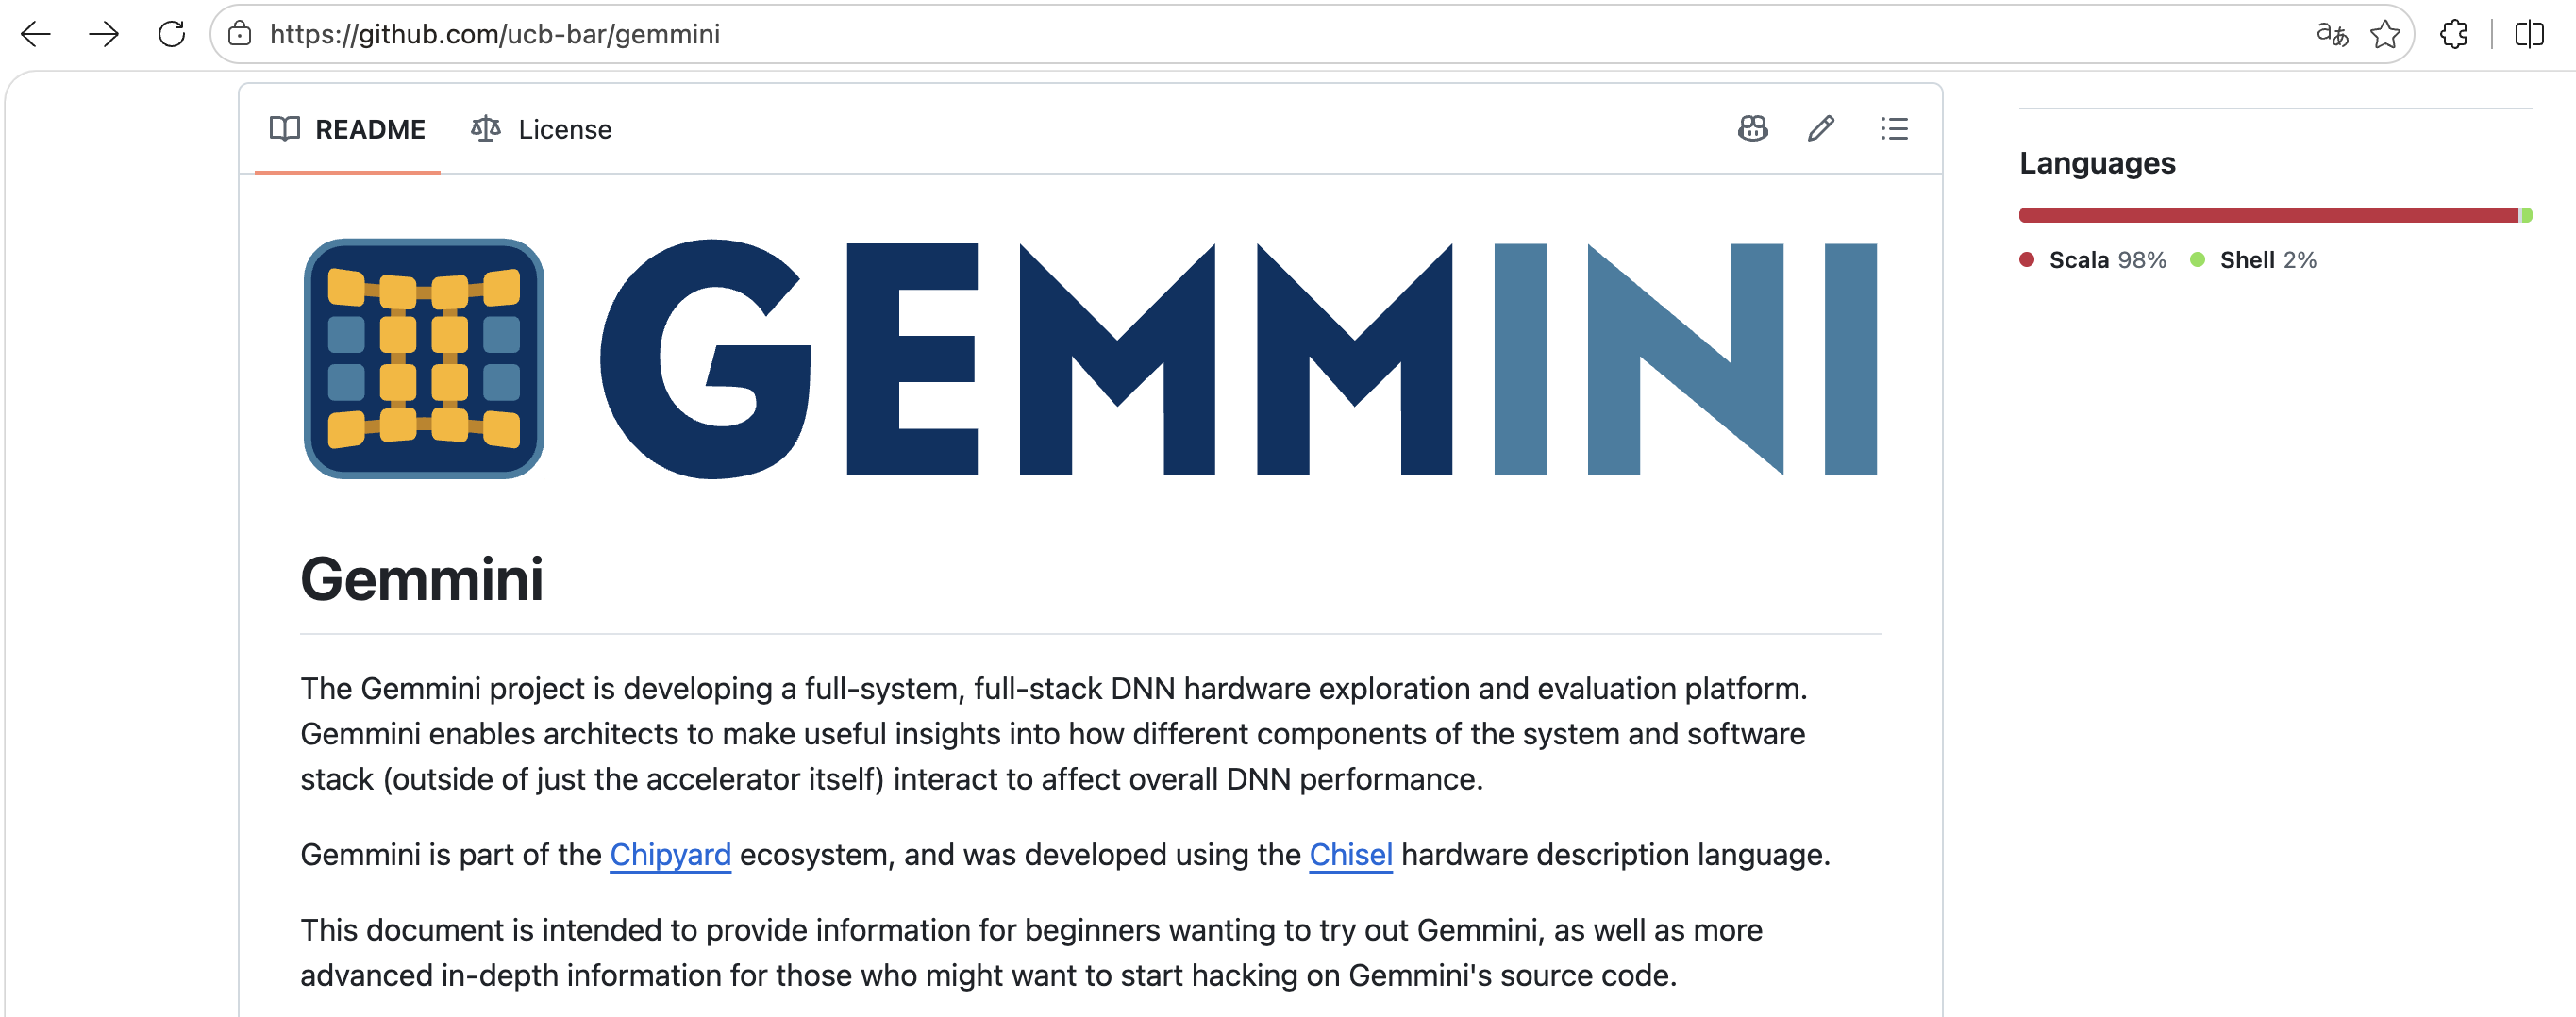
\includegraphics[width=.7\linewidth]{figures/03-arch/geminiWeb.png}
\caption{gemmini网页图}
\label{fig:08-gemmini-web}
\end{figure}



\subsection{Gemmini 开发环境部署}
\label{sec:08-gemmini-setup}

本教程从获取源码开始，直到 Chipyard 安装脚本成功结束并确认工具可用。
工程统一放在 \lstinline|~/SysArch/chipyard|，Conda 安装在
\lstinline|~/miniforge3|；其中 \lstinline|~| 表示当前用户的家目录，
不依赖用户名、服务器名称或共享磁盘位置。
本节不涉及 Gemmini 应用程序编译、RTL 仿真器构建、程序运行和性能测试。
安装脚本自身构建工具及预编译依赖的过程属于环境安装，仍需正常完成。

\paragraph{适用范围与准备条件}
Chipyard 官方主要在 x86 Linux 上开发和验证。本教程以采用 glibc 的
64 位 x86 Linux 为基准，建议使用 Ubuntu 22.04/24.04 或 Debian 12
这类常见开发系统；其他发行版需替换系统包管理命令。
不能仅凭使用 Linux 就保证完全兼容：Alpine 等 musl 系统、32 位系统
以及 ARM Linux 不属于本教程已经验证的适用范围。
ARM 主机还可能需要从源码构建 CIRCT，不能照搬 x86 的预编译包。
虚拟机也可以使用，但应分配足够的内存和磁盘。

需要能访问 GitHub（包括 Release 下载）、conda-forge 和 Maven 等依赖源。
建议预留至少 100 GiB 可用磁盘、16 GiB 内存；这只是完整安装的规划建议，
并非保证安装成功的最低配置。完整安装还包含 FireSim、FireMarshal 的相关依赖，
耗时和磁盘占用会随网络与机器配置变化。
无须提前安装 RISC-V 实体开发板、GPU 或 CUDA。
先用以下命令确认宿主机状况：

\begin{lstlisting}[language=bash]
uname -m
ldd --version | head -n 1
free -h
df -h ~
\end{lstlisting}

\lstinline|uname -m| 应显示 \lstinline|x86_64|。
以下所有命令均在 Bash 中依次执行；使用其他 Shell 的读者先执行
\lstinline|bash|。不要在 Conda 激活前启用 \lstinline|set -u|，
部分激活脚本会读取尚未定义的环境变量。

\paragraph{第一步：安装最初需要的系统工具}
Conda 会管理项目的大部分工具，但最初下载源码和安装器仍需系统提供
Git、curl、证书及基础构建工具。Ubuntu/Debian 使用：

\begin{lstlisting}[language=bash]
sudo apt-get update
sudo apt-get install -y git curl wget ca-certificates \
  bzip2 tar xz-utils patch build-essential
\end{lstlisting}

Fedora/RHEL 系发行版可对应使用以下命令；没有 sudo 权限时，请管理员安装
缺少的软件包，后面的工程与 Conda 安装均使用普通用户权限。

\begin{lstlisting}[language=bash]
sudo dnf install -y git curl wget ca-certificates \
  bzip2 tar xz patch gcc gcc-c++ make
\end{lstlisting}

不要同时执行两组包管理命令，也不要使用 sudo 运行后面的 Conda 和
Chipyard 安装脚本。

\paragraph{第二步：克隆 Chipyard 并固定版本}
Gemmini 已作为 Chipyard 的子模块管理，不需要再单独克隆一套独立工程。
为使本教程的步骤编号、依赖版本和恢复命令保持一致，使用与本次部署对应的
Chipyard 提交 \texttt{a7946ede}（版本描述为
\texttt{1.15.0-1-ga7946ede}）：

\begin{lstlisting}[language=bash]
mkdir -p ~/SysArch
cd ~/SysArch
git clone https://github.com/ucb-bar/chipyard.git
cd ~/SysArch/chipyard
git checkout --detach a7946ede
git describe --tags --always
\end{lstlisting}

此时出现 detached HEAD 提示是固定提交的正常结果。
若目标目录已经存在，应先确认它是否就是需要继续安装的工程，
不要删除已有源码或在含个人修改的工程中直接切换版本。
不要使用 \lstinline|git clone --recursive| 或手动初始化全部嵌套子模块；
由安装脚本选择并初始化项目所需的子模块。
以后更换 Chipyard 版本时，应重新核对对应版本的安装脚本，
不能假设步骤编号和工具版本始终不变。

\paragraph{第三步：安装并初始化 Miniforge}
Miniforge 提供 Conda；Chipyard 用它创建独立的项目环境。
如果已经在 \lstinline|~/miniforge3| 安装过可用的 Miniforge，
直接执行本段末尾的初始化命令，不要覆盖安装。
新安装时执行：

\begin{lstlisting}[language=bash]
mkdir -p ~/SysArch/downloads
cd ~/SysArch/downloads
curl -fL --retry 3 --connect-timeout 20 \
  -o Miniforge3-Linux-x86_64.sh \
  https://github.com/conda-forge/miniforge/releases/latest/download/Miniforge3-Linux-x86_64.sh
bash Miniforge3-Linux-x86_64.sh -b -p ~/miniforge3
\end{lstlisting}

随后在当前终端加载 Conda 并进入基础环境：

\begin{lstlisting}[language=bash]
source ~/miniforge3/etc/profile.d/conda.sh
conda activate base
conda --version
\end{lstlisting}

这里显式加载 \lstinline|conda.sh|，因此不要求提前执行
\lstinline|conda init| 或改写 \lstinline|~/.bashrc|。
如果已有 Miniconda/Miniforge 安装在其他位置，可以使用它，
但后续所有加载 Conda 的命令都必须统一为自己的安装位置。
本教程采用最新 Miniforge 引导安装器，具体项目依赖仍由固定提交中的
Conda 锁定文件决定；如需长期归档，应一并保存安装器及其校验值。

\paragraph{第四步：检查下载网络，按需设置代理}
可先检查源码站点的连接：

\begin{lstlisting}[language=bash]
curl -I -L --connect-timeout 15 --max-time 60 \
  https://github.com/ucb-bar/chipyard
\end{lstlisting}

能收到 HTTP 响应表示这一入口可达，不能据此推断所有依赖源均可下载。
如果网络可以直连，无需设置代理。需要代理时，使用自己机器可访问的代理地址，
不要照抄其他人的办公网 IP。以下仅以本机 SOCKS 服务监听 1080 端口为例，
端口和协议必须与自己的代理配置一致：

\begin{lstlisting}[language=bash]
export all_proxy=socks5h://127.0.0.1:1080
export ALL_PROXY="$all_proxy"
export http_proxy="$all_proxy"
export https_proxy="$all_proxy"
export HTTP_PROXY="$http_proxy"
export HTTPS_PROXY="$https_proxy"
export no_proxy=localhost,127.0.0.1
export NO_PROXY="$no_proxy"
\end{lstlisting}

\lstinline|socks5h| 表示通过代理解析域名。curl 支持该协议，但本版本
CIRCT 下载脚本使用的 wget 可能不支持；发生这一问题时按后面的恢复方法处理。
如果代理提供的是 HTTP 端口，应按代理软件说明使用
\lstinline|http://127.0.0.1:端口|，不能只把 SOCKS 地址的协议名改成 HTTP。
若 Conda、Git 或 Java 的下载仍超时，需分别检查它们的代理支持与配置。
代理环境变量只对当前终端及其启动的进程生效。

\paragraph{第五步：执行完整环境安装}
回到工程根目录，启用管道错误传递，并限制安装中遵守 Make 配置的任务并行度：

\begin{lstlisting}[language=bash]
source ~/miniforge3/etc/profile.d/conda.sh
conda activate base
cd ~/SysArch/chipyard
export MAKEFLAGS=-j4
set -o pipefail
./build-setup.sh riscv-tools
setup_status=$?
printf 'setup exit code: %s\n' "$setup_status"
\end{lstlisting}

\lstinline|MAKEFLAGS| 并不限制所有 Java、Conda 或脚本内部启动的任务。
内存较少时可改为 \lstinline|-j2|；不要根据服务器报告的全部 CPU 核数
盲目提高并行度。安装中应保持终端连接，可以使用自己熟悉的终端会话保持工具。
脚本已经自动把输出写入工程根目录的 \lstinline|build-setup.log|，
不必再向同一个文件添加外层 tee。

本版本完整安装的 11 个阶段依次为：
\begin{enumerate}
  \item 创建并安装项目 Conda 环境；
  \item 初始化 Chipyard 所需子模块；
  \item 安装工具链配套组件，包括 Spike、PK、libgloss 和 Gemmini 的 Spike 扩展；
  \item 生成源码导航标签；
  \item 预编译 Chipyard 的 Scala 依赖；
  \item 初始化 FireSim；
  \item 预编译 FireSim 的 Scala 依赖；
  \item 初始化 FireMarshal；
  \item 预构建 FireMarshal 的基础软件环境；
  \item 安装 CIRCT，其中包含 firtool；
  \item 执行仓库清理。
\end{enumerate}

本教程采用完整安装流程，与前面实际部署的步骤保持一致。
FireSim 和 FireMarshal 的初始化不意味着已经准备好 FPGA 云资源，
本节也不开展这些平台的后续使用。
\textbf{必须同时看到退出码为 0、日志中第 11 步结束以及
\lstinline|Setup complete!|，才能把安装脚本视为正常完成。}
只看到第 10 步下载结束还不够。

\paragraph{第六步：安装失败时从正确位置恢复}
先查看 \lstinline|~/SysArch/chipyard/build-setup.log| 的末尾，
确定失败阶段，不要反复删除整个工程。重新执行脚本会覆盖这份日志，
再次尝试前可在工程根目录保存副本：

\begin{lstlisting}[language=bash]
cd ~/SysArch/chipyard
cp build-setup.log "build-setup.$(date +%Y%m%d-%H%M%S).log"
tail -n 80 build-setup.log
\end{lstlisting}

若第 1 步已经成功，重新打开终端后先恢复项目环境：

\begin{lstlisting}[language=bash]
source ~/miniforge3/etc/profile.d/conda.sh
cd ~/SysArch/chipyard
source env.sh
\end{lstlisting}

\lstinline|-s N| 的含义是\textbf{跳过第 N 步}，不是从第 N 步开始。
只有确认此前阶段已经成功，才可以跳过它们；如果第 1 步环境创建本身不完整，
不能靠 \lstinline|-s 1| 掩盖错误，也不能仅因看到环境目录存在就认定安装成功。

\textbf{常见问题：第 10 步提示 Unsupported scheme。}
如果日志同时出现 \lstinline|socks5h://...: Unsupported scheme|、
\lstinline|gzip: stdin: unexpected end of file| 和 tar 错误，
通常是 wget 无法使用 SOCKS 代理，导致后续解压没有收到完整文件。
先确认 curl 能通过同一代理访问目标下载，再将本版本下载脚本中的 wget
替换为 curl：

\begin{lstlisting}[language=bash]
cd ~/SysArch/chipyard
sed -i.bak \
  's/wget -O - /curl -fL --retry 3 --connect-timeout 20 /' \
  tools/install-circt/bin/download-release-or-nightly-circt.sh
\end{lstlisting}

此命令适用于本教程固定版本的 Linux 脚本，原文件保存在同目录的
\lstinline|.bak| 文件中。若该行在其他版本中已经变化，需先查看脚本再修改。
不要额外下载一个任意版本的 firtool 来替换项目指定版本。
确认第 1--9 步均已成功后，执行以下命令\textbf{保留第 10、11 步}：

\begin{lstlisting}[language=bash]
source ~/miniforge3/etc/profile.d/conda.sh
cd ~/SysArch/chipyard
source env.sh
set -o pipefail
./build-setup.sh riscv-tools \
  -s 1 -s 2 -s 3 -s 4 -s 5 \
  -s 6 -s 7 -s 8 -s 9
setup_status=$?
printf 'setup exit code: %s\n' "$setup_status"
\end{lstlisting}

这里不能加 \lstinline|-s 11|，否则会跳过最后的清理阶段。
如果第 10 步已经成功、仅第 11 步未完成，则在上述命令末尾再加
\lstinline|-s 10|，只执行第 11 步。
下载超时、证书错误、磁盘不足和内存不足应分别处理；替换下载命令不能解决
所有网络或资源问题。

\paragraph{第七步：确认环境部署完成}
新终端中按固定顺序加载环境；以后进入本工程也使用这三条命令：

\begin{lstlisting}[language=bash]
source ~/miniforge3/etc/profile.d/conda.sh
cd ~/SysArch/chipyard
source env.sh
\end{lstlisting}

检查当前环境指向以及必要工具：

\begin{lstlisting}[language=bash]
printf 'CONDA_PREFIX=%s\nRISCV=%s\n' "$CONDA_PREFIX" "$RISCV"
conda env list
command -v riscv64-unknown-elf-gcc spike firtool
command -v verilator java sbt make
riscv64-unknown-elf-gcc --version | head -n 1
firtool --version
verilator --version
java -version
\end{lstlisting}

默认情况下，项目环境应位于 \lstinline|~/SysArch/chipyard/.conda-env|，
\lstinline|RISCV| 应指向该环境下的 \lstinline|riscv-tools|。
终端实际会显示展开后的家目录，这是正常现象。
编译器、Spike 和 firtool 应优先来自该项目环境，而非另一套系统安装。
本次部署的 firtool 为 1.75.0；版本要求以工程内
\lstinline|conda-reqs/circt.json| 为准，不以网上最新版本为准。
这里只检查版本，不启动 sbt，以免把环境验收变成额外的项目构建。

检查安装日志及 Gemmini 功能模型扩展：

\begin{lstlisting}[language=bash]
cd ~/SysArch/chipyard
tail -n 25 build-setup.log
if test -f "$RISCV/lib/libgemmini.so"; then
  echo 'Gemmini Spike extension exists'
  ldd "$RISCV/lib/libgemmini.so"
else
  echo 'Gemmini Spike extension is missing'
fi
\end{lstlisting}

动态依赖列表中不应出现 \lstinline|not found|；库文件缺失时应回看第 3 步，
而不是直接宣称 Gemmini 环境可用。
\textbf{验收结果应同时满足：安装脚本正常完成、项目环境加载正确、
必要工具可找到且能输出版本、Gemmini 扩展存在且依赖可解析。}
这些检查证明部署流程与基本工具就绪，并不等同于矩阵计算正确或 RTL 仿真通过。
到这里，本节的环境部署教程结束。

\paragraph{版本与资料来源}
安装步骤与恢复参数依据 Chipyard 提交 \texttt{a7946ede} 的安装脚本，
Gemmini 作为该提交锁定的子模块使用；Conda 引导方式参考 Miniforge 官方说明。
资料核对日期为 2026 年 11 月 25 日\cite{cysetup-a7946ede,cyinitial-a7946ede,miniforge-install}。
